\chapter{Introduction}

Automatic data processing and analysis is essential in many scientific disciplines and commercial
applications. The ever-increasing availability of computational resources experienced in recent
years has stimulated the establishment of new disciplines that strongly depend on analysis of massive
amounts of data. The complexity and scale of the data means that analysis by hand is often
impractical or even impossible. Therefore automatic processing by computational methods are of
paramount importance.

A clear example of this is found in biology. Methods to automate data acquisition have given rise to
powerful new techniques such as \emph{genome-wide association studies}, \emph{high-content
screening}, and \emph{gene expression profiling}. These techniques collect vast amounts of data that
must be carefully analyzed -- a task which would have been impossible to do by hand, just a few
years ago.

Recently, machine learning has become an essential step in the analysis process of many such
techniques.  Machine learning is a popular approach to automatic data processing and pattern
recognition that learns a predictive model from example data. Later, the predictive model can be
applied to new data for recognition or to make predictions. It is now common practice to use machine
learning to perform the analysis of many biological data sets because it is faster, more accurate,
and less biased than manual analysis.

Machine learning methods can be broadly categorized as either \emph{supervised} or
\emph{unsupervised}. Supervised methods are more widely used. They infer a predictive
model by detecting patterns in a set of labeled example data provided to the algorithm. Unsupervised
methods are designed to work without any training information. Clustering methods are a typical
example of unsupervised learning. 

In this work, we focus on supervised machine learning (SML) methods, which are designed to address
two families of problems: classification and regression. In the {\bf classification} problem,
instances of data (or objects) are said to belong to one class from a given set of classes. The task
is to assign unseen instances to the appropriate class. The {\bf regression} problem attempts to fit
a model to observed data in order to quantify the relationship between two groups of variables,
\emph{predictors} and \emph{responses}. The fitted model can be used to describe the relationship
between the two groups, or to predict new response values based on the predictor values.

% Talk about learning and prediction 


\subsubsection{Model selection}

Although many SML methods exist, it is usually not obvious which one to use. Choosing the best
algorithm for a particular problem can be difficult, even for an expert. There are several reasons
for this. First, the models underlying various machine learning algorithms are very different from
one another. In a simple example using toy data depicted in Figure \ref{fig:decision_boundaries}, the differences among 
various machine learning methods are obvious. Some methods misclassify entire regions of the data,
some perform well but generalize poorly (they overfit the data), and for some the decision boundary
is not smooth leading to ambiguity in certain regions.  

Unfortunately, there is no ``silver bullet'' machine learning algorithm that always performs well.  The choice of the method to use is tied to the structure of the data that they are to predict.  Some methods make assumptions on the
structure of the data, and do not give accurate predictions when such assumptions are violated. Therefore, it is important to choose the most appropriate model for the data, otherwise performance will suffer. 

\begin{figure}
	\begin{minipage}{0.33\textwidth}
		\centering
		\footnotesize \bf The \emph{two moon}\\classification problem.
		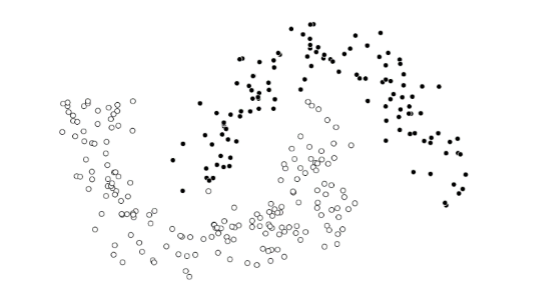
\includegraphics[width=\linewidth]{decision_boundaries1}
	\end{minipage}
	\begin{minipage}{0.33\textwidth}
		\centering
		\footnotesize {\bf $k$-nearest neighbors}\\($k=3$) ~ {\bf 99.6\%}
		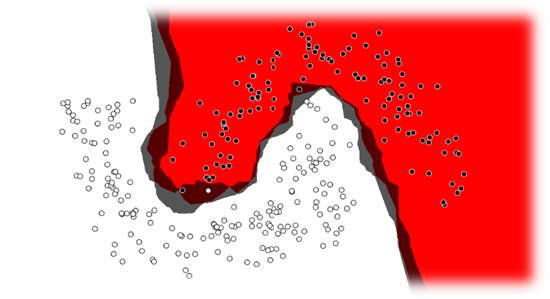
\includegraphics[width=\linewidth]{decision_boundaries2}
	\end{minipage}
	\begin{minipage}{0.33\textwidth}
		\centering
		\footnotesize {\bf Adaboost}\\with circular areas ~ {\bf 100\%}
		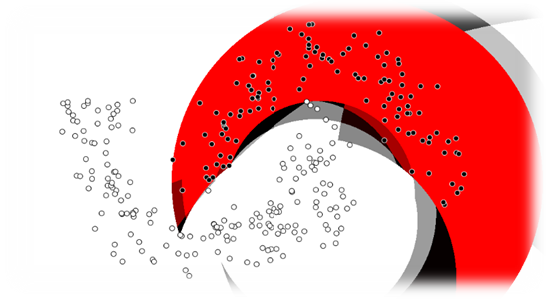
\includegraphics[width=\linewidth]{decision_boundaries3}
	\end{minipage}
	\begin{minipage}{0.33\textwidth}
		\centering
		\vskip0.5cm
		\footnotesize {\bf SVM}\\3$^{rd}$ order polynomial ~ {\bf 91.5\%}
		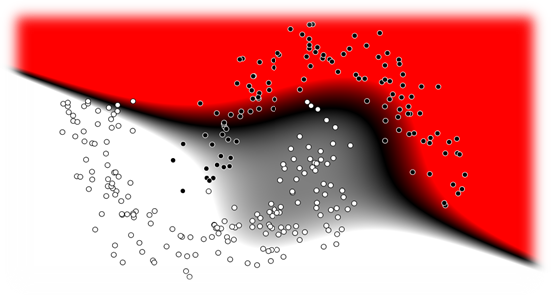
\includegraphics[width=\linewidth]{decision_boundaries4}
	\end{minipage}
	\begin{minipage}{0.33\textwidth}
		\centering
		\vskip0.5cm
		\footnotesize {\bf Neural network}\\(1 layer, 6 nodes) ~ {\bf 96.1\%}
		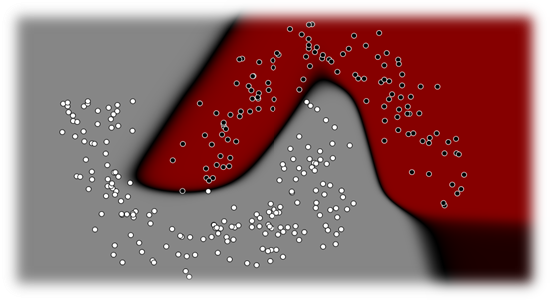
\includegraphics[width=\linewidth]{decision_boundaries5}
	\end{minipage}
	\begin{minipage}{0.33\textwidth}
		\centering
		\vskip0.5cm
		\footnotesize {\bf SVM}\\radial basis function ~ {\bf 100\%}
		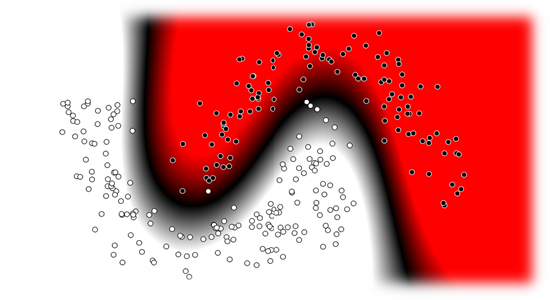
\includegraphics[width=\linewidth]{decision_boundaries6}
	\end{minipage}
	\caption[Decision boundaries for several different SML algorithms]{Decision boundaries for
	several different supervised machine learning algorithms applied to the \emph{two moon} dataset.
	Inherent differences among the various models are reflected in their performance and by the shape of the decision boundaries.}
	\label{fig:decision_boundaries}
\end{figure}

%The underlying rules learned by a SML algorithm, and used by it to map objects to values, is
%considered as a model of the object space. To select a SML model then means to evaluate a group of
%SML algorithms in order to choose the one that best maps objects to their target values.

\subsubsection{Hyperparameter optimization}

\emph{Hyperparameters} present a further complication to the problem. Most machine learning
algorithms contain hyperparameters, external settings left to be tuned by the user (as opposed to
parameters, which are optimized internally within the algorithm). These hyperparameter settings,
such as the cost of a support vector machine (SVM) or the number of neighbors $k$ in $k$-nearest
neighbors (KNN), control the SMLs internal behavior and can affect its ability to  learn patterns
for prediction. Finding the right combination of values may be as
critical to good prediction as selecting the right machine learning method.

The space of possible hyperparameters can be quite large. One common implementation of an SVM
requires the user to choose among 64 distinct categories of models, and then to set between 2 to 4
numeric values for each category. In many cases, an exhaustive evaluation of all possible
hyperparameter combinations is not practical, and it is often not even possible. In practice,
hyperparameter tuning is more of an art than a science, and even machine learning experts often
carry out the tuning in an arbitrary or subjective way.


\subsubsection{Our approach}

We present an automatic solution to the combined model selection and hyperparameter optimization problem. Model selection is the problem of determining which among a set of machine learning algorithms is the most well suited to the data, while hyperparameter optimization searches for candidate hyperparameter values expected to most improve the prediction of the SML algorithm.

Our approach is to organize the various machine learning algorithms and their hyperparameters into a large hierarchical space. At the lowest level of the hierarchy are the numeric hyperparameters which contain values that must be set appropriately. Up the hierarchy we model conditional and categorical choices, which all belong to a single family of machine learning algorithms (support vector machines, for example). We use numeric optimization methods at the lowest level to choose the best numeric hyperparameter values for a given categorical configuration. The candidate models compete against each other using statistical tests. The best candidates are promoted to the next level of the hierarchy. The process is repeated until ultimately a single model remains, chosen among the families of classifiers or regressors. 

Our approach substantially improves the performance of machine learning algorithms over their default settings, as we demonstrate on classic machine learning datasets as well as biological data. Our analysis also recognizes that, in some cases, the difference between one or more candidate models is statistically insignificant. When this occurs, the user can specify alternative criteria to choose the best model such as ranking the model's speed, simplicity, or interpretability.


%We approach it by evaluating of a series of candidate models in
%order to select the best one, according to some optimality criteria. 


%We do this with priority in computational resources given to more promising categories. 
